% !TEX root = notes.tex

\documentclass[9pt]{extarticle}

\usepackage[english]{babel}
\usepackage[utf8]{inputenc}
\usepackage[english]{babel}
\usepackage[dvipsnames]{xcolor}
\usepackage{geometry}
\usepackage{amsmath}
\usepackage{amssymb}
\usepackage{amsfonts}
\usepackage{amsthm}
\usepackage{ifthen}
\usepackage{makeidx}
\usepackage{hyperref}
\usepackage{parskip}
\usepackage{minted}
\usepackage{pgfplots}
\usepackage{siunitx}
\usepackage{marginnote}
\usepackage{graphicx}
\graphicspath{{./images/}}
% \usepackage[left=1cm,right=1cm]{geometry}
\usepackage{chngcntr}
\counterwithin{figure}{section}

\usetikzlibrary{calc}
\makeindex
\hypersetup{
    colorlinks,
    linktoc=all, 
    citecolor=black,
    filecolor=black,
    linkcolor=NavyBlue,
    urlcolor=black,
}
\usemintedstyle{arduino}
\pgfplotsset{width=10cm,compat=1.9}
\newif\ifediting%

\begin{document}

\newcommand{\sometext}{\bigskip\rm}
\newcommand{\eps}{\varepsilon}
\newcommand{\gradient}{\nabla}
\newcommand{\hessian}{\gradient^2}
\newcommand{\argmin}{\operatorname*{arg\,min}}
\newcommand{\argmax}{\operatorname*{arg\,max}}
% \newcommand{\R}[1][]{\mathbb{R}^{\ifx&#1&#1\else\fi}}
\newcommand{\R}{\mathbb{R}}
\newcommand{\Rn}{\mathbb{R}^n}
\newcommand{\Rm}{\mathbb{R}^m}
\newcommand{\Rnn}{\mathbb{R}^{n \times{} n}}
\newcommand{\Rnm}{\mathbb{R}^{n \times{} m}}
\newcommand{\Rmm}{\mathbb{R}^{m \times{} m}}
\newcommand{\C}{\mathbb{C}}
\newcommand{\iu}{\mathrm{i}\mkern1mu}
\newcommand{\eu}{\mathrm{e}\mkern1mu}
\newcommand{\boundary}{\partial}
\newcommand{\pathlength}{\mathrm{L}}
\newcommand{\sigmoid}{\sigma}
% \renewcommand{\qedsymbol}{}

% \swapnumbers
\theoremstyle{plain}
\newtheorem{theorem}{Theorem}[section]
\newtheorem{corollary}[theorem]{Corollary}
\newtheorem{lemma}[theorem]{Lemma}
\newtheorem{formulas}[theorem]{Formulas}
\newtheorem{algorithm}[theorem]{Algorithm}

\theoremstyle{definition}
\newtheorem{definition}[theorem]{Definition}
\newtheorem{definitions}[theorem]{Definitions}

% \theoremstyle{remark}
\newtheorem*{remark}{Remark}
\newtheorem*{remarks}{Remarks}
\newtheorem*{example}{Example}
\newtheorem*{examples}{Examples}
\newtheorem*{exercise}{Exercise}





\newpage
\thispagestyle{empty}
\begin{center}
    \quad \\[2cm] {\Large Notes on Math} \\[1cm]
\end{center}
\tableofcontents
\setcounter{page}{0}


\newcommand{\plotgoldensection}{%
	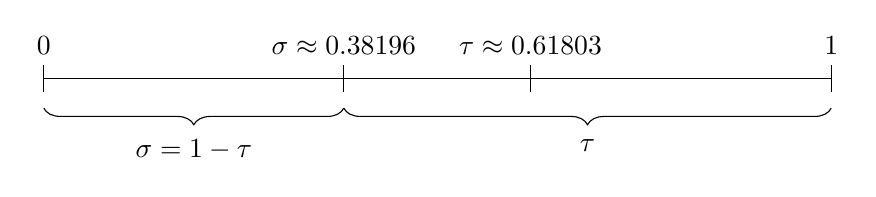
\begin{tikzpicture}
		\draw(0,0)--(10,0);
		\draw(0,-5pt)--(0,5pt) node[above] {$ 0 $};
		\draw(3.81,-5pt)--(3.81,5pt) node[above] {$ \sigma \approx 0.38196 $};
		\draw(6.18,-5pt)--(6.18,5pt) node[above] {$ \tau \approx 0.61803 $};
		\draw(10,-5pt)--(10,5pt) node[above] {$ 1 $};
		\draw[decorate, decoration={brace, mirror, amplitude=6pt}, yshift=-2.5ex] (0,0) -- node[below=1.8ex] {$ \sigma = 1 - \tau $} (3.81,0);
		\draw[decorate, decoration={brace, mirror, amplitude=6pt}, yshift=-2.5ex] (3.81,0) -- node[below=1.8ex] {$ \tau $} (10,0);
	\end{tikzpicture}
}

\newcommand{\plotsigmoid}{%
	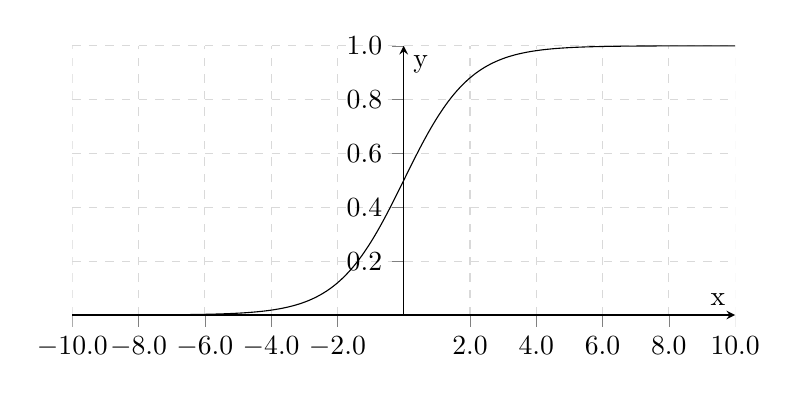
\begin{tikzpicture}
		\begin{axis}[
				legend pos=north west,
				axis x line=middle,
				axis y line=middle,
				x tick label style={/pgf/number format/fixed, /pgf/number format/fixed zerofill,
						/pgf/number format/precision=1},
				y tick label style={/pgf/number format/fixed, /pgf/number format/fixed zerofill,
						/pgf/number format/precision=1},
				grid = major,
				width=10cm,
				height=5cm,
				grid style={dashed, gray!30},
				xmin=-10,
				xmax= 10,
				ymin= 0,
				ymax= 1,
				axis background/.style={fill=white},
				xlabel=x,
				ylabel=y,
				tick align=outside,
				enlargelimits=false]
			\addplot[domain=-10:10,samples=500] {1/(1+exp(-x))};
			% \addlegendentry{$ \sigmoid(x) = \frac{1}{1+e^{-x}} $}
		\end{axis}
	\end{tikzpicture}
}

\newcommand{\plotvectorangle}{%
	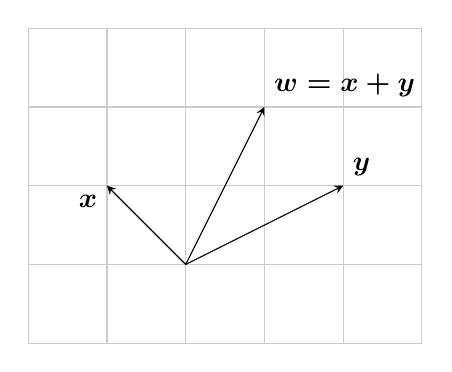
\begin{tikzpicture}
		\draw[thin,gray!40] (-2,-1) grid(3,3);
		\draw[-stealth](0,0) -- (-1,1) node[anchor=north east]{$\boldsymbol{x}$};
		\draw[-stealth](0,0) -- (2,1) node[anchor=south west]{$\boldsymbol{y}$};
		\draw[-stealth](0,0) -- (1,2) node[anchor=south west]{$\boldsymbol{w = x + y}$};
	\end{tikzpicture}
	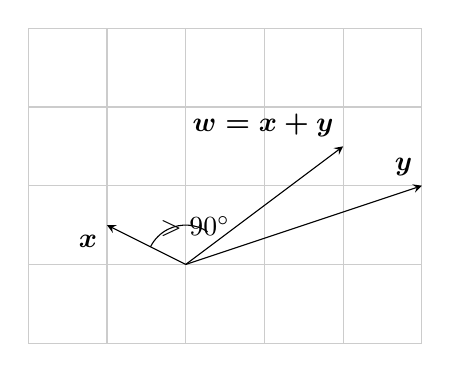
\begin{tikzpicture}
		\draw[thin,gray!40] (-2,-1) grid(3,3);
		\draw[-stealth](0,0) -- (-1,0.5) node[anchor=north east]{$\boldsymbol{x}$};
		\draw[-stealth](0,0) -- (3,1) node[anchor=south east]{$\boldsymbol{y}$};
		\draw[-stealth](0,0) -- (2,1.5) node[anchor=south east]{$\boldsymbol{w = x + y}$};
		\draw [black] (56.30:0.5) arc [start angle=56.30, end angle=153.43, radius=0.5cm]
		node [above right] {$ > \ang{90} $};
	\end{tikzpicture}
}


\newpage
\section{Minimization without Constraints}

Alternative proof of Lemma 2.10.

\lemma{}\label{lemma_gradient_inequality}
Let \(M \subseteq \mathbb{R}^n\) be a convex set and \(f \in C^1(M)\). Then \(f\) is convex if and only if
\[
    f(x) \ge f(y) + \gradient {f(y)}^T (x - y)
\]
for all \(x, y \in M \). 

\proof{}
Let f be convex and \(x, y \in M\). For \( 0 \le \lambda \le 1 \) we have
\[ 
    f(\lambda x + (1 - \lambda) y) \le \lambda f(x) + (1 - \lambda)f(y) =  \lambda f(x) - \lambda f(y) + f(y) 
\] 
and 
\[ 
    f(x) - f(y) \ge \frac{f(\lambda x + (1 - \lambda) y) - f(y)}{\lambda}
        = \frac{f(y + \lambda (x - y)) - f(y)}{\lambda}
\]
For \( d = x - y \)\ and \( \lambda \to 0 \) the term on the right converges to the direction derivative of \( f \)
in \( d \)
\[
    \frac{\partial f}{\partial d}(y) = \gradient{f(y)}^T d = \gradient{f(y)}^T (x - y) 
\]

Now let \( x, y \in M \) and  \( 0 \le \lambda \le 1 \). For \( z = \lambda x + (1 - \lambda) y \in M \) it follows that
\[
    \begin{split}
    \lambda f(x) & \ge \lambda f(z) + \lambda \gradient {f(z)}^T (x - z) \\
    (1 - \lambda) f(y) & \ge (1 - \lambda) f(z) + (1 - \lambda) \gradient {f(z)}^T (y - z)
    \end{split}
\]
Adding the two inequalities gives
\[
    \begin{split}
       \lambda f(x) + (1 - \lambda) f(y) 
        & \ge f(z) + \gradient {f(z)}^T(\lambda x - \lambda z + (1- \lambda) y - (1-\lambda)z) \\
        & = f(z) + \gradient {f(z)}^T(\lambda x + (1- \lambda) y - z) \\
        & = f(z)
    \end{split}
\]


\exercise{}
Let \( S \subset \mathbb{R}^n \) be compact and convex. Furthermore let \( f \in C^1(S) \) be convex,
\( x \in S \) and \( d \in \mathbb{R}^n \) a descent direction of \( f \) in \( x \) 
with \( \gradient {f(x)}^T d < 0 \).

\proof{}
If  \( x + \lambda^* d \) is an optimal solution then FONC holds and \( \gradient {f(x + \lambda^* d)}^T d = 0 \).
Let \( \gradient {f(x + \lambda^* d)}^T d = 0 \). Then Lemma\ref{lemma_gradient_inequality} gives
\[
    f(x + \lambda d) \ge f(x + \lambda^* d) + (\lambda - \lambda^*) \gradient {f(x + \lambda^* d)}^T d 
        = f(x + \lambda^* d) 
\]
and \( x + \lambda^* d \) is an optimal solution.



\newpage
\section{Nonlinear Optimization}
\subsection{Minimization without Constraints}
\bigskip


\begin{lemma}[Gradient Inequality]\label{thm:lemma_gradient_inequality}
    Let \(M \subseteq \mathbb{R}^n \) be a convex set and \(f \in C^1(M)\). Then \(f\) is convex if and only if
    \[
        f(x) \ge f(y) + \gradient {f(y)}^T (x - y)
    \]
    for all \(x, y \in M \).
\end{lemma}

\begin{proof}
    Let f be convex and \(x, y \in M\). For \( 0 \le \lambda \le 1 \) follows
    \[
        f(\lambda x + (1 - \lambda) y) \le \lambda f(x) + (1 - \lambda)f(y) =  \lambda f(x) - \lambda f(y) + f(y)
    \]
    and
    \[
        f(x) - f(y) \ge \frac{f(\lambda x + (1 - \lambda) y) - f(y)}{\lambda}
        = \frac{f(y + \lambda (x - y)) - f(y)}{\lambda}
    \]
    For \( d = x - y \)\ and \( \lambda \to 0 \) the term on the right converges to the direction derivative of \( f \)
    in \( d \)
    \[
        \frac{\partial f}{\partial d}(y) = \gradient{f(y)}^T d = \gradient{f(y)}^T (x - y)
    \]

    Now let \( x, y \in M \) and  \( 0 \le \lambda \le 1 \). For \( z = \lambda x + (1 - \lambda) y \in M \) 
    it follows that
    \[
        \begin{split}
            \lambda f(x) & \ge \lambda f(z) + \lambda \gradient {f(z)}^T (x - z) \\
            (1 - \lambda) f(y) & \ge (1 - \lambda) f(z) + (1 - \lambda) \gradient {f(z)}^T (y - z)
        \end{split}
    \]
    Adding the two inequalities gives
    \[
        \begin{split}
            \lambda f(x) + (1 - \lambda) f(y)
            & \ge f(z) + \gradient {f(z)}^T(\lambda x - \lambda z + (1- \lambda) y - (1-\lambda)z) \\
            & = f(z) + \gradient {f(z)}^T(\lambda x + (1- \lambda) y - z) \\
            & = f(z)
        \end{split}
    \]
\end{proof}
\bigskip


\begin{exercise}[Facility Locations]
    The facilities are located at:
    \[
        (3, 0), (0, -3), (1, 4)
    \]
\end{exercise}

\begin{proof}
    Let
    \[
        \begin{split}
            f(x)    & = {(x - 3)}^2 + y^2 + x^2 + {(y + 3)}^2 + {(x - 1)}^2 + {(y - 4)}^2 \\
            & = x^2 - 6x + 9 + y^2 + x^2 + y^2 + 6y + 9 + x^2 - 2x + 1 + y^2 -8y + 16 \\
            & = 3x^2 + 3y^2 - 8x - 2y + 35
        \end{split}
    \]
    Then
    \[
        \gradient f(x, y) = (6x - 8, 6y - 2) \text{ and } \gradient^2 f(x, y) =
        \begin{pmatrix}
            6 & 0 \\
            0 & 6 \\
        \end{pmatrix} > 0
    \]
    Hence \( (4 / 3, 1 / 3) \) is the gobal minimum.
\end{proof}
\bigskip


\exercise[Convex Functions]
The sum of convex functions is convex.

\proof{}
Let \( x, y \in M \). Since \( \alpha_i  > 0 \) it is
\[
    \begin{split}
        f(\lambda x + (1 - \lambda) y)
        & = \sum_{i=1}^m \alpha_i f_i(\lambda x + (1 - \lambda) y) \\
        & \le \sum_{i=1}^m \alpha_i \lambda f_i(x) + \sum_{i=1}^m \alpha_i (1 - \lambda) f_i(y)
        =  \lambda f(x) + (1 - \lambda) f(y)
    \end{split}
\]
Let \( f(x) = x^2 \). Then \( -f \) is not convex, e.g. \( x = 1, y = -1 \) and \( \lambda = 0.5 \).
\bigskip


\exercise[Solution of Quadratic Inequality]
Let
\[
    f(x) = x^{T}Ax + b^{T}x + c
\]
\proof{}
The product rule gives
\[
    \gradient {f(x)} = x^{T}A + Ax + b = (A^{T} + A)x + b = 2Ax + b
\]
Thus \( \hessian {f(x)} = 2A > 0 \) and \( f \) is convex. Hence the level set \( \Gamma_{-c} \) is convex.
Since the intersection of convex sets is convex \( \Gamma_{-c} \cap \{ x \in \Rn: g^{T}x + h = 0 \} \) 
is convex, too.
\bigskip


\exercise[Line Search on Compact Convex Sets]
Let \( S \subset \mathbb{R}^n \) be compact and convex. Furthermore let \( f \in C^1(S) \) be convex,
\( x \in S \) and \( d \in \mathbb{R}^n \) a descent direction of \( f \) in \( x \)
with \( \gradient {f(x)}^T d < 0 \).

\proof{}
If  \( x + \lambda^* d \) is an optimal solution then \( \gradient {f(x + \lambda^* d)}^T d = 0 \)
according to Theorem~\ref{thm:fonc}.
Let \( \gradient {f(x + \lambda^* d)}^T d = 0 \). Then Lemma~\ref{thm:lemma_gradient_inequality} gives
\[
    f(x + \lambda d) \ge f(x + \lambda^* d) + (\lambda - \lambda^*) \gradient {f(x + \lambda^* d)}^T d
    = f(x + \lambda^* d)
\]
and \( x + \lambda^* d \) is an optimal solution.
\bigskip


\begin{exercise}[Steepest Descent]
    Let
    \[
        f(x) = \frac{1}{2} x^T{A}x + b^T x + c
    \]
    where \( A \) is symmetrical and positive definite.
\end{exercise}

\begin{proof}
    Since \( \gradient {f(x)} = Ax + b \) and \( \hessian {f(x)} = A > 0 \) it follows \( x^* = -A^{-1}b \).
    Let \( v \) be eigenvector with \( Av = \mu v \). For \( x_0 = x^* + \theta v \) it follows
    \[
        \gradient {f(x_0)} = Ax^* + \mu \theta v + b = \mu \theta v
    \]
    and for \(\lambda \ge 0 \)
    \[
        \argmin \{ f(x_0 - \lambda \gradient f(x_0) \} =
            \argmin \{ f(x^* + \theta v - \lambda \mu \theta v)\} = \mu^{-1}
    \]
    Thus
    \[
        x_1 = x_0 - \mu^{-1} \gradient f(x_0) = x^* + \theta v - \mu^{-1} \mu \theta v = x^*
    \]
    and \( \gradient {f(x_1)} = 0 \). Hence the algorithm stops after the first iteration.
    Now let
    \[
        x_0 = x^* + \sum_{i=0}^m \theta_i v_i
    \]
    for orthogonal eigenvectors with \( Av_i = \mu_i\) and \( m \le n \). Then
    \[
        \gradient {f(x_0)} = Ax^* + \sum_{i=0}^m \mu_i \theta_i v_i + b = \sum_{i=0}^m \mu_i \theta_i v_i
    \]
    and
    \[
        x_1 = x_0 - \lambda \sum_{i=0}^m \mu_i \theta_i v_i
        = x^* + \sum_{i=0}^m \theta_i v_i - \lambda \sum_{i=0}^m \mu_i \theta_i v_i
        = x^* + \sum_{i=0}^m (1 - \lambda \mu_i) \theta_i v_i
    \]
    Since \( x^* \) is the minimum it follows \( \gradient {f(x_1)} = 0 \) iff \( \lambda = \mu^{-1} \) 
    for all \( 0 \le i \le m \).
\end{proof}
\bigskip



\subsection{One Dimensional Minimization and Direct Search}
\bigskip


\begin{definition}[Unimodal Function]\label{def:unimodal_fnc}
    A function \( f : [a,b] \to \R \) is called unimodal if there exists a \( \xi \in [a,b] \), so that
    \( f \) is strictly decreasing in \( [a, \xi] \) and strictly increasing in \( [\xi, b] \).
\end{definition}
\bigskip

In fact \( \xi \) is the unique minimum of \( f \) in \( [a, b] \). According to the definition,
for \( a \le x < y \le b \) follows
\[
    f(x) > f(y) \text{ for } x, y \in [a, \xi) \text{ and } f(x) < f(y) \text{ for }  x, y \in (\xi, b]   % chktex 9
\]
Thus
\[
    \xi \in [a, y] \text{ if } f(x) < f(y) \text{ and } \xi \in [x, b] \text{ if } f(x) \ge f(y)
\]

Consider now a symmetrical partioning of the interval \( [0, 1] \) where two consecutive partionings hold
the same ratio respectively:
\[
    \sigma = 1 - \tau \text{ and } \frac{1}{\tau} = \frac{\tau}{\sigma}
\]
Then \( 1 - \tau = \tau^2 \) and solving the quadratic equation \( \tau^2 + \tau = 1 \) yields
\[
    \tau = \frac{\sqrt{5} - 1}{2} \approx 0.61803
\]
\bigskip

\begin{figure}[H]
    \centering
    \plotgoldensection{}
    \caption{Golden Section}\label{fig:golden_section}
\end{figure}
\bigskip

Let now \( [a_0, b_0] = [a, b] \) and define
\[
    [a_{k + 1}, b_{k + 1}] =
    \begin{cases}
        [a_k, y_k] & \text{ if } f(x_k) < f(y_k)   \\
        [x_k, b_k] & \text{ if } f(x_k) \ge f(y_k)
    \end{cases}
\]
where
\[
    \begin{split}
        x_k & = b_k - \tau (b_k - a_k) \\
        y_k & = a_k + \tau (b_k - a_k)
    \end{split}
\]
It follows that \( [a_k, b_k] \supset [a_{k + 1}, b_{k + 1}] \) is a decreasing series of intervals with
\[
    (b_{k + 1} - a_{k + 1}) =  \tau(b_k - a_k)
\]
where the interval converges to \( \xi \). This leads to the following algorithm:
\bigskip

\begin{algorithm}[Golden Section Search]\label{algo:golden_section_search}
\end{algorithm}
\inputminted[fontsize=\small, framesep=0.35cm, frame=lines, python3=true]{python}{python/golden_section.py}
\bigskip

\begin{exercise}[Surprising Convergence]
    Example for \( f \in C^2(\mathbb{R}) \) with a sequence of strict local minima converging to a strict local maximum.
\end{exercise}
\bigskip



\subsection{Methods of Steepest Descent}
\bigskip


\begin{definition}
    Let \( f \in C^1(\Rn) \) and \( x_0 \in \Rn \) an arbitraty starting point.
    \begin{enumerate}
        \item For sequences \( \lambda_k > 0 \) and unit vectors \( s_k \in \Rn \) define
              \[
                  x_{k + 1} = x_k + \lambda_k s_k
              \]
        \item Assume there exists \( 0 < \alpha \le 1 \) so that
              \[
                  - \gradient f(x_k) s_k \ge \alpha \|\gradient f(x_k)\|
              \]
        \item Furthermore assume that for some \( 0 < \beta \le \gamma < 1 \) the following inequalities hold
              \[
                  f(x_{k + 1}) \le f(x_k) + \lambda_k \beta \gradient f(x_k) s_k
              \]
              \[
                  \gradient f(x_{k + 1}) s_k \ge \gamma \gradient f(x_k) s_k
              \]
    \end{enumerate}
    Then \( \lambda_k \) and  \( s_k \) are called \emph{step lengths} and \emph{search directions} respectively
    and \( x_k \) is called a \emph{sequence of descent} for \( f \).
\end{definition}
\bigskip


\begin{remarks}
    The inequalities above serve different purposes
    \begin{enumerate}
        \item  It is
              \[
                  - \gradient f(x_k) s_k = \cos\varphi \|\gradient f(x_k)\| \|s_k\| =
                  \cos\varphi \|\gradient f(x_k)\| \ge \alpha \|\gradient f(x_k)\|
              \]
              Hence the angle between the direction of the steepest descent and the search direction is
              strictly smaller then \( \ang{90} \) degrees.
        \item  Since \( \gradient f(x_k) s_k \le 0 \) it follows
              \[
                  f(x_{k + 1}) \le f(x_k) + \beta \lambda_k \gradient f(x_k) s_k \le f(x_k)
              \]
              and \( f(x_k) \) is monotonically decreasing.
        \item Furthermore
              \[
                  \gradient f(x_{k + 1}) s_k = \gradient f(x_k + \lambda_k s_k) s_k
                  \ge \gamma \gradient f(x_k) s_k
              \]
              Hence the step length cannot be chosen too small due to the continuity of the dervative.
    \end{enumerate}
\end{remarks}
\bigskip


\begin{theorem}[Steepest Descent Method]\label{thm:steepest_descent}
    Let \( f \in C^2(\Rn) \) and \( x_k \) a sequence of descent for \( f \).
    Then every accumulation point of \( x_k \) is a stationary point of \( f \).
\end{theorem}

\begin{proof}
\end{proof}


\newpage
\section{The Road to Reality}


\subsection{Hyperbolic Geometry}
The ratio between the area \( A \) and \( A' \) of two similar shapes is given by
\[
	A' = k^2A
\]
\bigskip

\begin{theorem}[Pythagoras]\label{thm:thm_pythagoras}
\[
    a^2 + b^2 = c^2
\]
\end{theorem}


\begin{proof}
Let \( A, B \) and \( C \) be the areas of the three triangles respectively. All triangles are similar, hence
\[
    B = \frac{b^2}{a^2} A \text{ and }  C =  \frac{c^2}{b^2} B 
\]
Since \( A + B = C \) it follows that
\[
     a^2 + b^2 = \frac{b^2A}{B} + b^2 = \frac{b^2(A + B)}{B} = \frac{b^2 C}{B} = c^2
\]
\end{proof}
\bigskip

% \begin{figure}[H]
% \centering
% \begin{tikzpicture}
% \rectriangle[black]{(0,0)}{(3,3)}{6cm}
% \end{tikzpicture}
% \caption{Pythagoras}\label{fig:pythagoras}
% \end{figure}
% \bigskip


\lemma[Conformal and Projective Representation]
The mapping from conformal and projective representation of any point is given by the radial expansion 
of the following factor
\[
   \frac{2R}{R^2 + r^2}
\]  

\begin{proof}
For any point the distance from the origin with regard to the two representations is given by
\[
    \log \frac{R + r}{R - r} = \frac{1}{2} \log \frac{R + r'}{R - r'} = \log \frac{(R + r')^2}{(R - r')^2}
\]
This gives
\[
  {(R - r)}^2 (R + r') = {(R + r)}^2 (R - r') \text{ and } -4R^2r + 2R^2r' + 2r^2r' = 0
\] 
Hence
\[
   r' = \frac{2R^2}{R^2 + r^2} r
\] 
\end{proof}


\subsection{Complex Numbers}

\begin{lemma}[Basic Formulas]\hfill
    \begin{enumerate}
        \item It is
            \[
                (a + \iu b) (c + \iu d) = (ac - bd) + \iu (ad + bc)
            \]
        \item Thus
            \[
               {(a + \iu b)}^2 = (a^2 - b^2) + \iu 2ab
            \]
            and
            \[
                (a + \iu b) (a - \iu b) =  a^2 + \iu ab - \iu ab - \iu^2b^2 = a^2 + b^2
            \]
        \item Hence
            \[
                \frac{a + \iu b}{c + \iu d} = \frac{(a + \iu b)(c - \iu d)}{c^2 + d^2} = 
                    \frac{ac + bd}{c^2 + d^2} + \iu \frac{bc - ad}{c^2 + d^2}
            \]
        \item For 
            \[
                z = \sqrt{\frac{1}{2}(a + \sqrt{a^2 + b^2})} + \iu \sqrt{\frac{1}{2}(-a + \sqrt{a^2 + b^2})} 
            \]
            it follows
            \[
                z^2 = \frac{1}{2}(a + \sqrt{a^2 + b^2}) - \frac{1}{2}(-a + \sqrt{a^2 + b^2}) +
                    \iu 2\sqrt{\frac{1}{4} (\sqrt{a^2 + b^2}^2) - a^2} = a + \iu b
            \]
    \end{enumerate}
\end{lemma}
\bigskip


\begin{lemma}[Binomial Theorem]\hfill
    \begin{enumerate}
        \item For the binomial coefficient Pascal's identity holds
			\[
				\binom{n}{k - 1} + \binom{n}{k} = \binom{n + 1 }{k }   
			\]  
        \item The following equation states the binomial identity
			\[
				{(a + b)}^n = \sum_{k=0}^{n} \binom{n}{k} a^{k} b^{n - k} = \sum_{k=0}^{n} \binom{n}{k} a^{n -k} b^{k}
			\]  
        \item For \( a = 1 \) follows
			\[
				{(1 + x)}^n = \sum_{k=0}^{n} \binom{n}{k} x^{k}
			\]  
    \end{enumerate}
\end{lemma}

\begin{proof}
It is
\[
	\binom{n}{k} + \binom{n}{k - 1} = \frac{n!}{k!(n - k)!} + \frac{n!}{(k - 1)!(n - k + 1)!}
		= \frac{n!(n + 1 - k) + n!k!}{k!(n + 1- k)!} = \binom{n + 1}{k}
\]
Furthermore by using induction
\[
    \begin{split}
		{(a + b)}^{n + 1}	& = \sum_{k=0}^{n} \binom{n}{k} a^{k + 1} b^{n - k} + 
								\sum_{k=0}^{n} \binom{n}{k} a^{k} b^{n + 1 - k} \\
							& = \sum_{k=1}^{n + 1} \binom{n}{k - 1} a^{k} b^{n + 1 - k} + 
								\sum_{k=0}^{n} \binom{n}{k} a^{k} b^{n + 1 - k} \\
							& = \sum_{k=0}^{n + 1} \binom{n + 1}{k} a^{k} b^{n + 1 - k}
    \end{split}
\]  
\end{proof}
\bigskip


\subsection{Exponential Function and Logarithms}

\begin{exercise}[Exponential Function]
The Cauchy product yields
\[
	\sum_{n=0}^\infty a_n \sum_{n=0}^\infty b_n = \sum_{n=0}^\infty \sum_{k=0}^n a_k b_{n-k}
\]  
if at least one of the series is absolutely convergent. Hence
\[
    \begin{split}
		\sum_{n=0}^\infty \frac{1}{n!} z^n \sum_{n=0}^\infty \frac{1}{n!} w^n 
			& = \sum_{n=0}^{\infty} \sum_{k=0}^{n} \frac{1}{k!} z^{k} \frac{1}{(n - k)!} w^{n - k} \\
			& = \sum_{n=0}^{\infty} \frac{1}{n!} \sum_{k=0}^{n} \binom{n}{k} z^{k}w^{n - k} \\
			& = \sum_{n=0}^\infty \frac{1}{n!} {(z + w)}^n	
    \end{split}
\]  
\end{exercise}
\bigskip


Let \( t \in \R \). Then
\[
    \begin{split}
		\eu^{\iu t}
			& = \sum_{k=0}^\infty \frac{1}{k!} {(\iu t)}^k \\
			& = \sum_{k=0}^\infty \frac{1}{2k!} {(\iu t)}^{2k} + 
				\sum_{k=0}^\infty \frac{1}{(2k + 1)!} {(\iu t)}^{2k + 1} \\
			& = \sum_{k=0}^\infty \frac{(-1)^k}{2k!} t^{2k} + 
				\iu\sum_{k=0}^\infty \frac{(-1)^k}{(2k + 1)!} t^{2k + 1} \\
			& = \cos{t} + \iu\sin{t}
    \end{split}
\]

More generally for \( z = \log r + \iu t\)
\[
	\eu^z = \eu^{\log r + \iu t} = r\eu^{\iu t} = r(\cos{t} + \iu\sin{t})
\]

For \( r = 1 \) and \( t = 2\pi \) this yields
\[
	\eu^{2\pi\iu} = \cos{2\pi} + \iu \sin{2\pi} = 1
\]
and for \( t = 2\pi \) we get
\bigskip

\begin{lemma}[Euler Equation]\label{lemma:lemma_euler_equation}
\[
	\eu^{\pi\iu} + 1 = 0
\]
\end{lemma}
\bigskip


\begin{exercise}\hfill
    \begin{enumerate}
        \item If \( \eu^z = w \) then \( z + \pi\iu \) is a logarithm to \( -w \):
			\( \eu^{z + \pi\iu} = \eu^{z}\eu^{\pi\iu} = - \eu^{z} = -w \).
		\item Since \( \eu^{i(s + t)} = \eu^{is} \eu^{it} \) it follows
			\[
				\begin{split}
					\cos{(s + t)} + \iu \sin{(s + t)} 
						& = (\cos{s} + \iu\sin{s})(\cos{t} + \iu\sin{t}) \\
						& = \cos{s}\cos{t} - \sin{s}\sin{t} + \iu(\cos{s}\sin{t} + \sin{s}\cos{t})
				\end{split}
			\]
			Hence
			\[
				\begin{split}
					\cos{(s + t)} & = \cos{s}\cos{t} - \sin{s}\sin{t} \\
					\sin{(s + t)} & = \cos{s}\sin{t} + \sin{s}\cos{t}
				\end{split}
			\]
		\item It is \( \eu^{3it} = (\eu^{it})^3 \) and thus
			\[
				\cos{3t} + \iu \sin{3t} 
					= (\cos{t} + \iu\sin{t})^3
					= \cos^3{t} - 3\cos{t}\sin^2(t) + \iu(\cos^2{t}\sin{t} -\sin^3{t})
			\]
        \item Fun facts
			\[ 
				\eu^{1 - 4\pi^2} = \eu^{1 + (2\iu\pi)^2} = \eu \eu^{2\pi\iu}\eu^{2\pi\iu} = \eu
			\]
			and \( \iu = \eu^{\iu\pi/2} \) gives
			\[
				\iu^\iu = \eu^{\iu\log\iu} = \eu^{\iu\iu\pi/2} = \eu^{-\pi/2} \in \R
			\]
    \end{enumerate}
\end{exercise}
\bigskip


\subsection{Complex Number Calculus}


\begin{theorem}[Cauchy Riemann Equations]\label{thm:thm_cauchy_riemann_eqations}
Let \( f = u + \iu v \) be holomorphic. Then \( f \) satisfies the Cauchy Riemann equations
\[
		\frac{\partial u}{\partial x} = \frac{\partial v}{\partial y}
\]
\[
		\frac{\partial u}{\partial y} = - \frac{\partial v}{\partial x}
\]
\end{theorem}

\begin{proof}
For \( h \in \R \) follows
\[
	\lim_{h \to 0}\frac{f(z + h) - f(z)}{h} = \frac{\partial u}{\partial x}(z) + \iu \frac{\partial v}{\partial x}(z)
\]	
and
\[
	\lim_{h \to 0}\frac{f(z + \iu h) - f(z)}{\iu h}
		= \frac{\partial u}{\iu\partial y}(z) + \frac{\partial v}{\partial y}(z)
		= \frac{\partial v}{\partial y}(z) - \iu\frac{\partial u}{\partial y}(z)
\]	

\end{proof}
\bigskip


\begin{exercise}\hfill
    \begin{enumerate}
        \item Let \( z_0 \in \C \) and \( \gamma(t) = z_0 + \eu^{\iu t} \) for \( t \in [0, 2\pi] \). Then
			\[
				\int_\gamma \frac{1}{z - z_0}\,dz 
					= \int_0^{2\pi} \frac{\iu \eu^{\iu t}}{z_0 + \eu^{\iu t} - z_0}\,dt
					= \int_0^{2\pi} \iu\,dt
					= 2\pi\iu
			\]
			and thus \( 1/ (z - z_0 ) \) is not holomorphic on \( \C \setminus \{z_0\} \)
    \end{enumerate}
\end{exercise}
\bigskip

\newpage
\section{Neural Networks}

\subsection{The Perceptron}

\begin{definition}[Binary Classifiers]
    Let \( X \subset \R^n \) be the union of two finite disjoint sets \( X = M \cup N \).
    \begin{enumerate}
        \item A \emph{binary classification problem} is the task to find a mapping \( f: X \to \{ 0, 1 \} \) with
              \[
                  f(x) = \left \{
                  \begin{array}{ll}
                      1 & \text{ for } x \in M \\
                      0 & \text{ for } x \in N
                  \end{array}
                  \right.
              \]
              \( f \) then is called a \emph{binary classifier} for \( X \)
        \item \( X \) is called \emph{separable} if there exists a \emph{weight vector} \( w \in \R^n \)
              and a \emph{bias} \( b \in \R \) so that
              \[
                  \begin{split}
                      wx + b & > 0 \hspace{1em}\text{ for } x \in M \\
                      wx + b & < 0 \hspace{1em}\text{ for } x \in N
                  \end{split}
              \]
        \item The weight \( w \) and the bias \( b \) are called \emph{solution to the classification problem}.
              They implicitly define a binary classifier via
              \[
                  f(x) = \left \{
                  \begin{array}{ll}
                      1 & \text{ if } wx + b > 0 \\
                      0 & \text{ if } wx + b < 0
                  \end{array}
                  \right.
              \]
    \end{enumerate}
\end{definition}
\bigskip


\begin{examples}
    \hfill
    \begin{enumerate}
        \item Let \( X = \{ 0, 1 \} \times \{ 0, 1 \} \) and consider the \emph{and} operator
              \( f(1, 1) = 1 \) and \( f(x, y) = 0 \) elsewhere. Then \( w = (3, 3) \) and \( b = -5 \)
              yield a solution to the classification problem \( M = f^{-1}(1) \) and \( N = f^{-1}(0) \)
        \item Again let \( X = \{ 0, 1 \} \times \{ 0, 1 \} \) and \( f(1, 0) = f(0, 1) = 1 \) and
              \( f(0, 0) = f(1, 1) = 0 \), the \emph{xor} operator. Thus for any weight \( (w_1, w_2) \) and
              any bias \( b \)
              \[
                  \begin{split}
                      w_1 + b & > 0 \\
                      w_2 + b & > 0 \\
                      \\
                      w_1 + w_2 + b & \le 0 \\
                      b & \le 0
                  \end{split}
              \]
              Adding two equations respectively shows that there is no solution
        \item The bias can be integrated into the weight vector via \( w' = (w, b) \in \R^{n + 1} \) and
              \( x' = (x, 1) \in \R^{n + 1} \). Separability then reduces to
              \[
                  w'x' > 0
              \]
    \end{enumerate}
\end{examples}
\bigskip


\subsubsection*{Geometrical Interpretation}
The idea for the perceptron most likely has its origin in a simple geometrical observation.
Recall that for \( x, y \in \R^n \) the dot product can be expressed as
\[
    xy = \|x\| \|y\| \cos\alpha
\]
where \( \alpha \) is the angle between the two vectors. Hence the product is positive
if the angle is less than \( \ang{90} \) degrees and negative if the angle is between \( \ang{90} \)
and \( \ang{180} \) degrees
\[
    \begin{split}
        xy & > 0 \hspace{1em}\text{ for } 0 \le \alpha < \pi / 2 \\
        xy & < 0 \hspace{1em}\text{ for } \pi / 2 < \alpha \le \pi
    \end{split}
\]
Note, that the sign does not depend on the vector lengths, but solely on the angle.

For any two vectors it is easy enough to find a weight that satisfies \( wx > 0 \) and \( wy > 0 \).
Generally \( w = x + y \) is a good guess, but not always correct as shown below in
\hyperref[fig:vectorangle]{Figure~\ref*{fig:vectorangle}}.

\bigskip
\begin{figure}[H]
    \centering
    \plotvectorangle{}
    \caption{Dot Product and Angle}\label{fig:vectorangle}
\end{figure}
\bigskip

But, the more similar the lengths of the two vectors are the more likely \( x + y \) works.
An iterative approach is to increase \( w = x + y \) in the direction of vector with the angle greater
than \( \ang{90} \) degrees.
\[
    w_{n + 1} = \left \{
    \begin{array}{ll}
        w_n + x & \text{ if } w_n x < 0 \\
        w_n + y & \text{ if } w_n y < 0 \\
    \end{array}
    \right.
\]
\bigskip

\begin{examples}
    \hfill
    \begin{enumerate}
        \item Let \( x = (-1, 1) \) and \( y = (6, 1) \). Then
              \[
                  \begin{aligned}
                      w_0 & = (5, 2) & w_0x & = -3 & w_0y & = 32 \\
                      w_1 & = (4, 3) & w_1x & = -1 & w_1y & = 27 \\
                      w_2 & = (3, 4) & w_2x & = 1  & w_2y & = 22 \\
                  \end{aligned}
              \]
        \item Let \( x = (4, -6) \) and \( y = (-10, 5) \). Then
              \[
                  \begin{aligned}
                      w_0 & = (-6, -1)  & w_0x & = -18 & w_0y & = 55  \\
                      w_1 & = (-2, -7)  & w_1x & = 34  & w_1y & = -15 \\
                      w_2 & = (-12, -2) & w_2x & = -36 & w_2y & = 110 \\
                      w_3 & = (-8, -8)  & w_3x & = 16  & w_3y & = 40  \\
                  \end{aligned}
              \]
        \item Let \( \|x\| < \|y\| \) and \( \cos\alpha < 0 \). Then
              \[
                  \begin{split}
                      x(x + y) & = xx + xy = {\|x\|}^2 + \|x\| \|y\| \cos\alpha \\
                      x(x + y) & = \|x\| \|x + y\| \cos\beta
                  \end{split}
              \]
              and
              \[
                  {\|x + y\|}\cos\beta = \|x\| + \|y\|\cos\alpha > 0
              \]
              Hence \( \cos\beta > 0 \) if
              \[
                  \|x\| > -\|y\|\cos\alpha
              \] 
    \end{enumerate}
\end{examples}
\bigskip

\begin{algorithm}[Weight]\label{algo:weight}
\end{algorithm}
\inputminted[fontsize=\small, framesep=0.35cm, frame=lines, python3=true]{python}{python/weight.py}
\bigskip



\begin{algorithm}[Perceptron]\label{algo:perceptron}
\end{algorithm}
\inputminted[fontsize=\small, framesep=0.35cm, frame=lines, python3=true]{python}{python/perceptron.py}
\bigskip


\subsection{The Backtracking Algorithm}

\begin{definition}[Activation Functions]
    \hfill
    \begin{enumerate}
        \item The \emph{Heaviside} function \( H: \R \to \{ 0, 1 \} \) is defined as
              \[
                  H(x) = \left \{
                  \begin{array}{ll}
                      1 & \text{ for } x > 0  \\
                      0 & \text{ for }x \le 0
                  \end{array}
                  \right.
              \]
        \item The \emph{sigmoid} function \( \sigmoid \in C^\infty(\R) \) is defined as
              \[
                  \sigmoid(x) = \frac{1}{1 + e^{-x}}
              \]
    \end{enumerate}
\end{definition}
\bigskip


\begin{figure}[H]
    \centering
    \plotsigmoid{}
    \caption{The sigmoid function \( \sigmoid(x) = \frac{1}{1 + e^{-x}} \)}\label{fig:sigmoid}
\end{figure}
\bigskip


\begin{remarks}
    \hfill
    \begin{enumerate}
        \item Since the heaviside function is not continuous and therefore not differentiable at \( 0 \)
              the sigmoid function is often considered its smooth counterpart
        \item The definition of the sigmoid function yields \( 0 < \sigmoid(x) < 1 \) as well as
              \( \sigmoid(x) \to 0 \) for \( x \to -\infty \) and \( \sigmoid(x) \to 1 \) for \( x \to \infty \)
        \item The quotient rule yields
              \[
                  \sigmoid'(x)
                  = -\frac{-e^{-x}}{{(1 + e^{-x})}^2}
                  = \sigmoid(x) \frac{1 + e^{-x} - 1}{1 + e^{-x}}
                  = \sigmoid(x)(1 - \sigmoid(x))
              \]
              and \( \sigmoid \) is monotonically increasing over its domain
    \end{enumerate}
\end{remarks}
\bigskip

\newpage
\section{Neural Networks}

\subsection{The Perceptron}
\bigskip

\begin{definition}[Binary Classifiers]
    Let \( X \subset \R^n \) be the union of two finite disjoint sets \( X = M \cup N \).
    \begin{enumerate}
        \item A \emph{binary classification problem} is the task to find a mapping \( f: X \to \{ 0, 1 \} \) with
              \[
                  f(x) = \left \{
                  \begin{array}{ll}
                      1 & \text{ for } x \in M \\
                      0 & \text{ for } x \in N
                  \end{array}
                  \right.
              \]
              \( f \) then is called a \emph{binary classifier} for \( X \)
        \item \( X \) is called \emph{separable} if there exists a \emph{weight vector} \( w \in \R^n \)
              and a \emph{bias} \( b \in \R \) so that
              \[
                  \begin{split}
                      wx + b & > 0 \hspace{1em}\text{ for } x \in M \\
                      wx + b & < 0 \hspace{1em}\text{ for } x \in N
                  \end{split}
              \]
        \item The weight \( w \) and the bias \( b \) are called \emph{solution to the classification problem}.
              They implicitly define a binary classifier via
              \[
                  f(x) = \left \{
                  \begin{array}{ll}
                      1 & \text{ if } wx + b > 0 \\
                      0 & \text{ if } wx + b < 0
                  \end{array}
                  \right.
              \]
    \end{enumerate}
\end{definition}
\bigskip


\begin{examples}
    \hfill
    \begin{enumerate}
        \item Let \( X = \{ 0, 1 \} \times \{ 0, 1 \} \) and consider the \emph{and} operator
              \( f(1, 1) = 1 \) and \( f(x, y) = 0 \) elsewhere. Then \( w = (3, 3) \) and \( b = -5 \)
              yield a solution to the classification problem \( M = f^{-1}(1) \) and \( N = f^{-1}(0) \)
        \item Again let \( X = \{ 0, 1 \} \times \{ 0, 1 \} \) and \( f(1, 0) = f(0, 1) = 1 \) and
              \( f(0, 0) = f(1, 1) = 0 \), the \emph{xor} operator. Thus for any weight \( (w_1, w_2) \) and
              any bias \( b \)
              \[
                  \begin{split}
                      w_1 + b & > 0 \\
                      w_2 + b & > 0 \\
                      \\
                      w_1 + w_2 + b & \le 0 \\
                      b & \le 0
                  \end{split}
              \]
              Adding two equations respectively shows that there cannot be a solution
        \item The bias can be integrated into the weight vector via \( w' = (w, b) \in \R^{n + 1} \) and
              \( x' = (x, 1) \in \R^{n + 1} \). Separability then reduces to
              \[
                  w'x' > 0
              \]
    \end{enumerate}
\end{examples}
\bigskip


\subsubsection*{Geometrical Interpretation}
\bigskip
The idea for the perceptron most likely has its origin in a simple geometrical observation.
Recall that for \( x, y \in \R^n \) the dot product can be expressed as
\[
    xy = \|x\| \|y\| \cos\alpha
\]
where \( \alpha \) is the angle between the two vectors. Hence the product is positive
if the angle is less than \( \ang{90} \) degrees and negative if the angle is between \( \ang{90} \)
and \( \ang{180} \) degrees
\[
    \begin{split}
        xy & > 0 \hspace{1em}\text{ for } 0 \le \alpha < \pi / 2 \\
        xy & < 0 \hspace{1em}\text{ for } \pi / 2 < \alpha \le \pi
    \end{split}
\]
Note, that the sign does not depend on the vector lengths, but solely on the angle.

For any two vectors it is easy enough to find a weight that satisfies \( wx > 0 \) and \( wy > 0 \).
Generally \( w = x + y \) is a good guess, but not always correct as shown below in
\hyperref[fig:vectorangle]{Figure~\ref*{fig:vectorangle}}.

\bigskip
\begin{figure}[H]
    \centering
    \plotvectorangle{}
    \caption{Dot Product and Angle}\label{fig:vectorangle}
\end{figure}
\bigskip

But, the more similar the lengths of the two vectors are the more likely \( x + y \) works.
The actual threshold is given by the following
\bigskip

\begin{lemma}
    Let \( x, y \in \Rn \) with \( \|x\| < \|y\| \) and \( xy = \|x\| \|y\| \cos\alpha \). If
    \[
        \|x\| > -\|y\|\cos\alpha
    \]
    then \( x(x + y) > 0 \).
\end{lemma}

\begin{proof}
    Let \( x(x + y) = \|x\| \|x + y\| \cos\beta \). Since
    \[
        x(x + y) = xx + xy = {\|x\|}^2 + \|x\| \|y\| \cos\alpha
    \]
    it follows
    \[
        {\|x + y\|}\cos\beta = \|x\| + \|y\|\cos\alpha
    \]
    Hence \( \cos\beta > 0 \) if the inequality above holds.
\end{proof}
\bigskip


An iterative approach is to repeatedly increase \( w = x + y \) in the direction of the shorter vector
aka the one with the angle greater than \( \ang{90} \) degrees.
\[
    w' = \left \{
    \begin{array}{ll}
        w + x & \text{ if } w x \le 0 \\
        w + y & \text{ if } w y \le 0 \\
    \end{array}
    \right.
\]

While this seems reasonable it is unclear whether the algorithm always yields a result after
a finite number of iterations. The answer to this question will be given later as a special case
of the \hyperref[thm:perceptron_convergence]{Perceptron Convergence Theorem~\ref*{thm:perceptron_convergence}}.

This approach can be used to to separate two vectors. Finding a common weight for  \( x \) and \( -y \)
now yields \( wx > 0 \) and \( -wy > 0 \), hence \( wy < 0 \).
\[
    w' = \left \{
    \begin{array}{ll}
        w + x & \text{ if } w x \le 0 \\
        w - y & \text{ if } w y \ge 0 \\
    \end{array}
    \right.
\]
\bigskip


\begin{algorithm}[Weight]\label{algo:weight}
\end{algorithm}
\inputminted[fontsize=\small, framesep=0.35cm, frame=lines, python3=true]{python}{python/weight.py}
\bigskip


\begin{examples}
    \hfill
    \begin{enumerate}
        \item Let \( x = (-1, 1) \) and \( y = (6, 1) \). Then
              \[
                  \begin{aligned}
                      w_0 & = (5, 2) & w_0x & = -3 & w_0y & = 32 \\
                      w_1 & = (4, 3) & w_1x & = -1 & w_1y & = 27 \\
                      w_2 & = (3, 4) & w_2x & = 1  & w_2y & = 22 \\
                  \end{aligned}
              \]
        \item Let \( x = (4, -6) \) and \( y = (-10, 5) \). Then
              \[
                  \begin{aligned}
                      w_0 & = (-6, -1)  & w_0x & = -18 & w_0y & = 55  \\
                      w_1 & = (-2, -7)  & w_1x & = 34  & w_1y & = -15 \\
                      w_2 & = (-12, -2) & w_2x & = -36 & w_2y & = 110 \\
                      w_3 & = (-8, -8)  & w_3x & = 16  & w_3y & = 40  \\
                  \end{aligned}
              \]
        \item Task: for any given integer \( k \) find two vectors so that more than \( k \) steps are needed
        \item Let \( w = x / \|x\| + y/ \|y\| \). Then
              \[
                  wx = \frac{{\|x\|}^2}{\|x\|} + \frac{yx}{\|y\|} = \|x\| + \|x\|\cos\alpha = (1 + \cos\alpha)\|x\| > 0
              \]
              and on the other hand \( wx = \|w\| \|x\| \cos\beta \). Similarily
              \( wy = (1 + \cos\alpha)\|y\| = \|w\| \|y\| \cos\gamma \). Hence
              \[
                  1 + \cos\alpha = \|w\|\cos\beta = \|w\|\cos\gamma
              \]
              and thus \( \beta = \gamma \). Also, as expected, \( wx > 0 \) and \( wy > 0 \)
    \end{enumerate}
\end{examples}
\bigskip


The following theorem is the generalization of the approach above for binary classifiers.
Roughly sepaking the algorithm changes the weight only for misqualified vectors. The proof measures
the change of angle against the change of length of the weight vector and provides an estimation
for the maximumn number of required steps.
\bigskip

\begin{theorem}[Perceptron Convergence Theorem]\label{thm:perceptron_convergence}
    Let \( X = M \cup N \) be separable by \( w^*\in \Rn \). Define \( w_0 = 0 \)
    and repeat to iterate over all \( x \in X \) via
    \[
        w_{k + 1} = \left \{
        \begin{array}{ll}
            w_k + x & \text{ if } x \in M \text{ and } w_k x \le 0 \\
            w_k - x & \text{ if } x \in N \text{ and } w_k x \ge 0 \\
            w_k     & \text{ else }                                \\
        \end{array}
        \right.
    \]
    until no further changes occurr. Suppose \( \|x\| \le r \)  and \( |w^*x| \ge \delta > 0 \)
    for \( x \in X \). Then the number of iterations before the algorithm stops is limited by
    \[
        k\le \frac{r^2}{\delta^2}
    \]
\end{theorem}

\begin{proof}
    Let \( x \in M \) with \( w_k x \le 0 \). Then
    \[
        w^*w_{k + 1} = w^*w_k + w^*x \ge w^*w_k + \delta
    \]
    Furthermore
    \[
        \|w_{k + 1}\|^2 = \|w_k + x\|^2 = \|w_k\|^2 + 2w_k x + \|x\|^2 \le \|w_k\|^2 + r^2
    \]

    The same estimations holds for \( x \in N \) with \( w_k x \ge 0 \) and using induction yields
    \[
        w^*w_k \ge k\delta \text{ and } \|w_k\|^2 \le kr^2
    \]
    Assuming \( \|w^*\| = 1\) now gives
    \[
        k^2\delta^2 \le \|w_k\|^2 \le kr^2
    \]
    which proves the initial inequality.
\end{proof}
\bigskip


\begin{algorithm}[Perceptron]\label{algo:perceptron}
\end{algorithm}
\inputminted[fontsize=\small, framesep=0.35cm, frame=lines, python3=true]{python}{python/perceptron.py}
\bigskip


\begin{remark}
    Check \hyperref[thm:banach_fix_point]{Banach Fixed-Point Theorem~\ref*{thm:banach_fix_point}}
    for an alternative proof?!
\end{remark}
\bigskip


\subsection{Single Layer Feedforward Neural Networks and the Delta Rule}
\bigskip

\begin{definition}[Activation Function]
    \hfill
    \begin{enumerate}
        \item There is no valuable formal definition for an \emph{activation function}
              \( \alpha: \R \to Y \subseteq \R \). However, the behaviour of an activation function should
              somehow relate to the fireing behaviour of an actual biological neuron. Continuity,
              differentiability, monotony and the behaviour at infinity are of special interest in order
              to apply mathematical concepts
        \item An activation function \( \alpha: \R \to \R \) with \( \alpha(x) \to 0 \)
              for \( x \to -\infty \) and \( \alpha(x) \to 1 \) for \( x \to \infty \) is called a
              \emph{sigmoidal activation function}
        \item The \emph{Heaviside} function \( H: \R \to \{ 0, 1 \} \) is defined as
              \[
                  H(x) = \left \{
                  \begin{array}{ll}
                      1 & \text{ for } x > 0  \\
                      0 & \text{ for }x \le 0
                  \end{array}
                  \right.
              \]
        \item The \emph{sigmoid} function \( \sigmoid \in C^\infty(\R) \) is defined as
              \[
                  \sigmoid(x) = \frac{1}{1 + e^{-x}}
              \]
    \end{enumerate}
\end{definition}
\bigskip


\begin{remarks}
    \hfill
    \begin{enumerate}
        \item The heaviside function is not continuous and therefore not differentiable at \( 0 \).
              In that sense the sigmoid function can be considered its smooth counterpart
        \item The definition of the sigmoid function yields \( 0 < \sigmoid(x) < 1 \) as well as
              \( \sigmoid(x) \to 0 \) for \( x \to -\infty \) and \( \sigmoid(x) \to 1 \)
              for \( x \to \infty \)
        \item The quotient rule yields
              \[
                  \sigmoid'(x)
                  = -\frac{-e^{-x}}{{(1 + e^{-x})}^2}
                  = \sigmoid(x) \frac{1 + e^{-x} - 1}{1 + e^{-x}}
                  = \sigmoid(x)(1 - \sigmoid(x))
              \]
              and \( \sigmoid \) is monotonically increasing over its domain
    \end{enumerate}
\end{remarks}
\bigskip


\begin{figure}[H]
    \centering
    \plotsigmoid{}
    \caption{The sigmoid function \( \sigmoid(x) = \frac{1}{1 + e^{-x}} \)}\label{fig:sigmoid}
\end{figure}
\bigskip

\begin{remarks}
    \hfill
    \begin{enumerate}
        \item Let \( f \in C^1(\Rn) \) and \( g(x) = f(x|^2 \). The multivariable  chain rule yields
              \[
                  \frac{\partial g}{\partial x_i}(x)
                  = \frac{\partial f^2}{\partial x_i}(x)
                  = 2 f(x) \frac{\partial f}{\partial x_i}(x)
              \]
              and
              \[
                  \gradient g(x) = 2 f(x) \gradient f(x)
              \]
        \item More generally for \( f = (f_1, f_2, \dots f_n)\in C^1(\Rn,\Rm) \) and
              \[
                  g(x) = \|f(x)\|^2 = \sum_{j = 1}^m {f_j(x)}^2
              \]
              it follows that
              \[
                  \frac{\partial g_j}{\partial x_i}(x)
                  = \sum_{j = 1}^m \frac{\partial f_j^2}{\partial x_i}(x)
                  = 2 \sum_{j = 1}^m \frac{\partial f_j}{\partial x_i}(x) f_j(x)
              \]
              and
              \[
                  \gradient g(x) = 2 \sum_{j = 1}^m \gradient f_j(x) f_j(x)
              \]
        \item Now let \( x \in \Rn \) and \( y \in R \) be fixed. For \( q(w, b) = wx + b - y \) follows
              \[
                  \begin{split}
                      \frac{\partial q}{\partial w_i}(w, b) &=
                      \frac{\partial}{\partial w_i} \sum_{i = 0}^n w_i x_i + b - y = x_i \\
                      \frac{\partial q}{\partial b}(w, b) &= 1
                  \end{split}
              \]
              Hence
              \[
                  \gradient q(w, b) = (x_1, x_2, \dots, x_n, 1)
              \]
        \item Let \( \alpha \in C^1(\R) \) be an activation function and define
              \( p(w,b) = (y - \alpha(wx + b))^2 \).
              Then
              \[
                  \begin{split}
                      \frac{\partial p}{\partial w_i}(w, b) &= -2 (y - \alpha(wx + b)) \alpha'(wx + b) x_i  \\
                      \frac{\partial p}{\partial b}(w, b) &= -2 (y - \alpha(wx + b)) \alpha'(wx + b)
                  \end{split}
              \]
              and
              \[
                  \gradient p(w, b) = -2 (y - \alpha(wx + b)) \alpha'(wx + b)\gradient q(w, b)
              \]
    \end{enumerate}
\end{remarks}
\bigskip


\begin{definition}[Single Layer Feedforward Neural Network]
    Let \( \alpha \in C^1(\R) \) be an activation function, \( w \in \R^n \)  and \( b \in \R \)
    be weight and bias. Define \( f \in C^1(\Rn) \) as
    \[
        f(x) = \alpha(w x + b)
    \]
    Then \( f = \alpha(wx + b) \) is called a \emph{single layer feedforward neural network}.
\end{definition}
\bigskip


\begin{definition}[Error Function]
    Let \( f = \alpha(wx + b) \) be a single layer feedforward neural network.
    \begin{enumerate}
        \item A finite set \( T \subset \Rn \times \R \) is called  \emph{test set}
        \item The \emph{error function} is defined as the mean squared error over the samples
              \[
                  E(w,b) = \frac{1}{2} \sum_{(x,y) \in T} {(y - f(x))}^2
              \]
    \end{enumerate}
\end{definition}
\bigskip


\begin{lemma}
    It is
    \[
        \begin{split}
            \frac{\partial E}{\partial w_i}(w, b) &= \sum_{(x,y) \in T} - (y - f(x)) \alpha'(wx + b) x_i\\
            \frac{\partial E}{\partial b}(w, b) &= \sum_{(x,y) \in T} - (y - f(x)) \alpha'(wx + b)
        \end{split}
    \]
\end{lemma}

\begin{proof}
    This follows from the remarks above.
\end{proof}
\bigskip


The Delta Rule applies the method of the Steepest Descent to the error function of a neural network.
\bigskip


\begin{algorithm}[Delta Rule]\label{algo:delta_rule}
    Let \( f = \alpha(wx + b) \) be a single layer feedforward neural network
    and \( T \) a test set.
    The delta rule modifies weight and bias in the direction of the greatest descent \( - \eta \gradient E(w,b) \)
    at a given \emph{learning rate} \( \eta > 0 \).  For \( (x, y) \in T \) this is
    \[
        \begin{split}
            \Delta w_i & = \eta (y - f(x)) \alpha'(wx + b) x_i \\
            \Delta b & = \eta (y - f(x)) \alpha'(wx + b)
        \end{split}
    \]
\end{algorithm}
\bigskip


\inputminted[fontsize=\small, framesep=0.35cm, frame=lines, python3=true]{python}{python/delta_rule.py}
\bigskip


\subsection{The Univeral Approximation Theorem}
\bigskip

% \begin{definition}[Single Layer Neural Network]
%     Let \( w_k \in \R^n \) and \( b_k \in \R \). For \( \alpha_k \in \R \) define \( f : \Rn \to \R \)
%     \[
%         f(x) = \sum_{k = 0}^m \alpha_k \sigmoid(w_k x + b_k)
%     \]
%     Then \( f \) is called a \emph{single layer feedforward neural network} of \( m \) units.
% \end{definition}
% \bigskip

\begin{theorem}[The Universal Approximation Theorem]\label{thm:universal_approximation}
    The subspace of all single layer feedforward neural networks is dense in \( C(I^n) \).
\end{theorem}


%\subsection{The Backpropagation Algorithm}

\end{document} 
